% §4 The axiom scheme and the classical affine theory --- blueprint chapter 4
% (blueprint/src/parts/04-classical.tex). Written from the draft's §4 (Q-0287, 2026-10-04), on the
% template of sections 2 and 3 (Q-0285, Q-0286). Every statement is transcribed verbatim from its
% node under a `% shared with blueprint` marker, with the paper statement's \label equal to the
% blueprint label (records/affine/transcribe-shared-statements.py), so that `linkage check` reports
% it `verbatim`. Two statements were changed at the blueprint first, in the safe direction, and
% re-transcribed: lem:operators-to-kernels(4)-(5) (draft numbers removed) and
% thm:cascade-infinitely-divisible(3)(c) (a justification by a section-5 node moved to the proof).
%
% Order. The blueprint's: the scheme and the passage from operators (4.1), the parameter space
% (4.2), the null array (4.3), the single step and rigidity (4.4); then the prior art and the
% relation to the line (4.5), which has no node. The draft put lem:operators-to-kernels before
% def:affine-cascade-family; the lemma's clause (4) names the definition, so it follows it here.
%
% Forward references. Two proofs rest on section 5 (prop:isotropic-corner on the ray families of
% 5.6, thm:cascade-infinitely-divisible(3)(c) on the stable step cone of 5.5), as the blueprint's
% forward edges do; nothing there uses section 4's nodes in return. Section 5 is written in
% parallel (Q-0288), so its labels are not \ref'd here (`linkage paper` would fail on them): the
% proofs restate what they take and point to \S\ref{sec:landscape}. When both sections are merged,
% those pointers may become \ref's to the nodes (prop:gw-ray-families(1) and (3),
% lem:gw-kernels-from-origin(1)-(2), prop:similarity-ray-families(3), prop:stable-step-cone(2)),
% which also clears the `[uses]` advisories of the two proofs.
%
% Proofs. The proofs of record are the blueprint's. Short ones are transcribed; long ones are
% shortened to their decisive steps and headed "Sketch" (section 1.1's convention). A cited fact is
% named by its number and its \ref, with no page anchor (section 2.6 holds them). The prior-art
% remarks follow the reading notes records/affine/READING-{kelker1970distribution,
% fang1990symmetric,skitovich1954linear,comon1994independent,lindeberg2011generalized}.md.
%
% After the blind review (Q-0289; records/affine/REVIEW-paper-section-4.md): two more statements
% changed at the blueprint and re-transcribed (def:gw-cascade-family and
% lem:operators-to-kernels(1), "the single-operator axioms other than (A3)";
% thm:cascade-infinitely-divisible(3)(c) split into three sentences). The neighbours of 4.5 follow
% READING-{lindeberg1997shape-affine,alvarez1993axioms,pauwels1995extended,duits2004axioms}.md.
% Table 4.1 and Figure (fig-rank-deficient-step.png, records/affine/fig-rank-deficient-step.py) are
% review flag 39's. The shared-text flags marked "can wait" are listed in GATE-section-4.md.
%
% Shortened into Appendix B (Q-0291, the author's decision of 2026-10-04, as Q-0290 did for
% section 5; records/affine/move-sections-3-4-to-appendices*.py): lem:operators-to-kernels moved
% whole (no later argument here consumes it; 4.1 says what it gives), and the proofs of 4.1-4.4
% verbatim but for their headings, except those of thm:rank-deficient-step and thm:affine-rigidity;
% the second paragraph of rem:kelker became rem:no-covariance there. Every other statement stays.

\section{The axiom scheme and the classical affine theory}\label{sec:classical}

In dimension $d \ge 2$ an aperture has a shape as well as a size, and the scalar parameter of the
line becomes a matrix $\Sigma$, proportional to the covariance of the aperture in the Gaussian case.
Its size, the scale, is the part that the dilations move. Two
structures then act on the parameter. A group $G$ of linear maps of the image moves it by
$A \cdot \Sigma = A\Sigma A^{\tp}$, and the family is required to be covariant under $G$. Covariance is
what lets a measurement at one shape be carried to another by the image's own change of
coordinates, the use of shape adaptation (\S\ref{sec:landscape-uses}). An order $W$ on the matrices says
along which pairs the family cascades, so that a coarser record is a further smoothing of a finer
one.

The section has two aims. The first is to state the axioms once, for every pair $(G, W)$, so that
each case of the classification of \S\ref{sec:landscape} is an instance of one definition
(\S\ref{sec:affine-covariance}). The second is the theorem at the classical end of that
classification: with the general linear group and the Loewner order, one rank-deficient step of the
cascade forces the Gaussian (Theorem~\ref{thm:affine-rigidity}, \S\ref{sec:affine-single-step}). That
theorem is the reference point from which \S\ref{sec:landscape} measures what a smaller group or a
smaller order buys. Between the two, two subsections settle what every case shares and what the
rest of the paper uses. The first explains why the positive definite matrices $\PD(d)$ index the
kernels. For $\GL(d)$ the axioms supply a rotation-invariant kernel $\mu_I$, and every kernel from
scale zero at a positive definite matrix is a linear image of it (\S\ref{sec:parameter-space}). The second shows that along every order with a path
condition each increment is infinitely divisible (Theorem~\ref{thm:cascade-infinitely-divisible},
\S\ref{sec:null-array}). Every increment then has a generating triplet, a Gaussian covariance, a
\Levy{} measure and a drift, and \S\ref{sec:landscape} reads the families through those triplets.
The section closes with the prior art and the relation to the line (\S\ref{sec:classical-prior-art}).

\subsection{The \texorpdfstring{$(G, W)$}{(G, W)} scheme, from operators to kernels}\label{sec:affine-covariance}

This subsection states the axioms for every pair $(G, W)$, on operators and on kernels
(Definition~\ref{def:gw-cascade-family}), as the line paper and the isotropic paper state theirs
(Definitions~\ref{def:line-family} and~\ref{def:isotropic-kernel-family}). The operator form is
where the axioms have their meaning as measurements, and the kernel form is where the proofs are
done. The kernel form for the general linear group with the Loewner order, the classical case, is
written out as Definition~\ref{def:affine-cascade-family}. Three statements then serve every pair: a
family whose kernels from scale zero have transforms without zeros is determined by them
(Lemma~\ref{lem:gw-kernels-from-origin}), along rays these
kernels are exactly the covariant fields of self-decomposable laws
(Proposition~\ref{prop:gw-ray-families}), and on the multiples of $I$ the similarities with the ray
order give, up to a change of the scale coordinate, the isotropic theory
(Proposition~\ref{prop:isotropic-corner}).

The group must contain the dilations, so that zooming the image is always a change of parameter. The
order must contain the rays, so that blurring an aperture without changing its shape is always a
step of the cascade. With a matrix as parameter, the paper uses two concepts, one from matrix analysis
and one from the Lie theory of semigroups. The first is the \emph{Loewner order}: $\Sigma \le \Sigma'$
when $\Sigma' - \Sigma$ is positive semidefinite, that is, when
$\langle w, \Sigma w\rangle \le \langle w, \Sigma' w\rangle$ for every $w \in \RR^d$
(\sscite{hilgert1997causal}, Ex.~2.2.3, p.~41). For apertures it says that the aperture of
$\Sigma'$ is at least as wide as that of $\Sigma$ in every direction
(Figure~\ref{fig:rank-deficient-step}). Scale-space theory uses it already. The Gaussian kernels form
a semigroup over covariance matrices: the kernel of $\Sigma_1$ convolved with that of $\Sigma_2$ is the
kernel of $\Sigma_1 + \Sigma_2$ (\sscite{lindeberg1994scale}, (15.34)--(15.35), p.~391). Lindeberg's
cascade over covariance matrices requires the difference $\Sigma' - \Sigma$ to be positive semidefinite
(\sscite{lindeberg2013computational}, fn.~7, p.~594), and the increment of the affine Gaussian scale
space from $\Sigma$ to $\Sigma'$ is the Gaussian with covariance $2b(\Sigma' - \Sigma)$
(Definition~\ref{def:affine-cascade-family}). The second concept is the \emph{wedge} of Hilgert,
Hofmann and Lawson, a closed convex set that contains $0$ and is closed under addition
(\sscite{hilgert1989lie}, p.~3). For the orders of this paper the steps of $W$ between positive
definite matrices are generated by such a cone of symmetric matrices (\S\ref{sec:invariant-wedges}),
although Definition~\ref{def:gw-cascade-family} does not require one. The pair $(G, W)$ is called a
\emph{wedge datum} after its order.

% shared with blueprint def:gw-cascade-family
\begin{definition}[the $(G, W)$ cascade scheme]\label{def:gw-cascade-family}
Fix an integer $d \ge 1$. Write $\PSD(d)$ for the real symmetric positive semidefinite
$d \times d$ matrices and $\PD(d) \subseteq \PSD(d)$ for the positive definite ones. The group
$\GL(d)$ acts on $\PSD(d)$ by $A \cdot \Sigma := A\Sigma A^{\tp}$, on probability measures on
$\RR^d$ by pushforward, $A_*\mu := \mu \circ A^{-1}$, and on $L^1(\RR^d)$ by
$D_Af := |\det A|^{-1}f(A^{-1}\,\cdot)$; with
$\widehat\mu(\omega) = \int e^{i\langle\omega,x\rangle}\mu(dx)$ one has
$\widehat{A_*\mu}(\omega) = \widehat\mu(A^{\tp}\omega)$. A \emph{wedge datum in dimension $d$} is a
pair $(G, W)$ of
\begin{itemize}
\item a closed subgroup $G$ of $\GL(d)$ containing the dilations $\lambda I$, $\lambda > 0$, and
\item a partial order $\le_W$ on $\PSD(d)$ that is \emph{$G$-invariant}, $\Sigma \le_W \Sigma'$
implying $A \cdot \Sigma \le_W A \cdot \Sigma'$ for every $A \in G$, and \emph{contains the rays},
$c\,\Sigma \le_W c'\,\Sigma$ whenever $\Sigma \in \PSD(d)$ and $0 \le c \le c'$.
\end{itemize}
Write $P_W$ for the set of pairs $(\Sigma, \Sigma')$ with $\Sigma \le_W \Sigma'$, with the topology
of $\PSD(d) \times \PSD(d)$. Since $W$ contains the rays, $0 \le_W \Sigma$ for every $\Sigma$, and
in particular $(0, I) \in P_W$.
\begin{enumerate}
\item \emph{(Operator form.)} A \emph{$(G, W)$-cascade family of operators} is a family
$(\Phi_{\Sigma,\Sigma'})_{(\Sigma,\Sigma') \in P_W}$ of linear operators on the real space
$L^1(\RR^d)$ such that
\begin{enumerate}
\item[(A1)] each $\Phi_{\Sigma,\Sigma'}$ is a bounded operator on $L^1(\RR^d)$;
\item[(A2)] each $\Phi_{\Sigma,\Sigma'}$ commutes with the translations $T_af := f(\cdot - a)$,
$a \in \RR^d$;
\item[(A4)] each $\Phi_{\Sigma,\Sigma'}$ maps nonnegative functions to nonnegative functions;
\item[(A5)] each $\Phi_{\Sigma,\Sigma'}$ preserves $\int f$ for $f \ge 0$;
\item[(A6)] \emph{(cascade)} $\Phi_{\Sigma,\Sigma} = \mathrm{Id}$ and
$\Phi_{\Sigma',\Sigma''}\Phi_{\Sigma,\Sigma'} = \Phi_{\Sigma,\Sigma''}$ whenever
$\Sigma \le_W \Sigma' \le_W \Sigma''$;
\item[(A7)] \emph{(continuity)} for every $f \in L^1(\RR^d)$ the map $(\Sigma,\Sigma') \mapsto \Phi_{\Sigma,\Sigma'}f$
is continuous from $P_W$ into $L^1(\RR^d)$;
\item[(ND)] \emph{(nondegeneracy)} $\Phi_{0,I} \ne \mathrm{Id}$;
\item[(Cov)] \emph{(covariance)} $D_A\Phi_{\Sigma,\Sigma'}D_A^{-1} = \Phi_{A\cdot\Sigma,\,A\cdot\Sigma'}$ for every
$A \in G$ and every $(\Sigma,\Sigma') \in P_W$.
\end{enumerate}
Axioms (A1), (A2), (A4) and (A5) are the single-operator axioms of
\restated{V}{Def.~3.1}{def:line-family} other than the reflection axiom (A3), read in $\RR^d$.
\item \emph{(Kernel form.)} A \emph{$(G, W)$-cascade family of kernels} is a family
$(\mu_{\Sigma,\Sigma'})_{(\Sigma,\Sigma') \in P_W}$ of probability measures on $\RR^d$ such that
\begin{enumerate}
\item[(K1)] \emph{(cascade)} $\mu_{\Sigma,\Sigma} = \delta_0$, and
$\mu_{\Sigma,\Sigma''} = \mu_{\Sigma',\Sigma''} * \mu_{\Sigma,\Sigma'}$ whenever
$\Sigma \le_W \Sigma' \le_W \Sigma''$;
\item[(K2)] \emph{(continuity)} for every $\omega \in \RR^d$ the map
$(\Sigma,\Sigma') \mapsto \widehat\mu_{\Sigma,\Sigma'}(\omega)$ is continuous on $P_W$;
\item[(K3)] \emph{($G$-covariance)} $A_*\mu_{\Sigma,\Sigma'} = \mu_{A\cdot\Sigma,\,A\cdot\Sigma'}$ for
every $A \in G$ and every $(\Sigma,\Sigma') \in P_W$;
\item[(K4)] \emph{(nondegeneracy)} $\mu_{0,I} \ne \delta_0$.
\end{enumerate}
We write $\mu_\Sigma := \mu_{0,\Sigma}$ for the \emph{kernel from scale zero}.
\end{enumerate}
The \emph{Loewner order}, $\Sigma \le \Sigma'$ when $\Sigma' - \Sigma \in \PSD(d)$, and the
\emph{ray order}, under which $\Sigma$ precedes $\Sigma'$ when $\Sigma = 0$ or $\Sigma' = c\,\Sigma$
for some $c \ge 1$, contain the rays and are invariant under every subgroup of $\GL(d)$. The
\emph{corners} of the scheme are these four data:
\begin{itemize}
\item the similarities $\{cQ : c > 0,\ Q \in \Orth(d)\}$ with the ray order, read on the multiples
$sI$, $s \ge 0$, of the identity (the isotropic theory);
\item $(\GL(d), \text{Loewner})$, the classical case, whose kernel form is
Definition~\ref{def:affine-cascade-family};
\item $(\GL(d), \text{rays})$;
\item the similarities with the Loewner order.
\end{itemize}
\end{definition}

% Round 3 (content review), B.R5: the corners are inside Definition 3.1, which is set upright.
Four data recur throughout, and the definition ends by listing them as the corners of
the scheme. They are the reference points of the landscape. In Table~\ref{tab:landscape} they are
the cells of the general linear and the similarity rows in the ray and the Loewner columns. The
isotropic theory (\S\ref{sec:iso-recap}) is the first, read on the multiples of $I$
(below, and Proposition~\ref{prop:isotropic-corner} in Appendix~\ref{app:classical}). The classical
theory of this section is the second. The third and the fourth are the two ends of the landscape of \S\ref{sec:landscape}. The
ray order is the smallest order that contains the rays, and $(\GL(d), \text{rays})$ pairs it with
the largest group. The similarities with the Loewner order pair the smaller group of the four with
the larger order.

The two forms correspond axiom by axiom. The single-operator axioms (A1), (A2), (A4) and (A5) make
each $\Phi_{\Sigma,\Sigma'}$ convolution by a probability measure $\mu_{\Sigma,\Sigma'}$, its kernel,
as on the line (Lemma~\ref{lem:line-representation}). Then (A6) corresponds to (K1), (A7) to (K2), (Cov) to (K3) and (ND) to (K4). The line's axiom (A8) leaves the
relabelling of the scales free; the scheme fixes the action of the group on the parameter,
$A \cdot \Sigma$, and for $\GL(d)$ on $\PD(d)$ a relabelling that commutes with that action is a
constant multiple (Lemma~\ref{lem:affine-gauge}). The passage from operators to kernels is
Lemma~\ref{lem:operators-to-kernels}, the line's Lemma~\ref{lem:line-representation} proved again in
$\RR^d$ with balls for intervals; its clause (5) gives the same passage for the isotropic families.
Its converse is Lemma~\ref{lem:kernels-to-operators}: convolution with the kernels of a family
satisfies the operator axioms. Both are stated and proved in Appendix~\ref{app:classical}. So the
two forms describe the same families, and the theory proceeds on kernels from here
(\S\ref{sec:introduction}, ``Scope'').

Nondegeneracy is required at the one pair $(0, I)$ only.
Asking it at every pair would exclude a family of the similarities with the ray order whose
kernels at the singular matrices are trivial (Appendix~\ref{app:classical}, after
Proposition~\ref{prop:isotropic-corner}).
% Round 3 (content review), B.S4 (the author's decision D12, second part;
% VERIFY-round3-front-classical-paper.md B.S4, delta_at_pd_family-output.txt): what (K4) at one pair allows.
For the same corner it also allows the kernel $\delta_0$ at a positive definite aperture. The centred
Gaussian kernels with covariance $\phi(\Sigma)\tr(\Sigma)\,I$, $\Sigma \ne 0$, and $\delta_0$ at $0$, form such
a family when $\phi \ge 0$ is a continuous function of the eigenvalues of $\Sigma$ divided by its
trace, positive at $I$ and zero at some positive definite matrix
(Proposition~\ref{prop:gw-ray-families}(2)).

The proofs of \S\ref{sec:affine-single-step} work with the kernel form at the classical corner, so
it is written out once.

% shared with blueprint def:affine-cascade-family
\begin{definition}[affine cascade family]\label{def:affine-cascade-family}
Fix an integer $d \ge 1$, and let $\PSD(d)$, $\PD(d)$, the Loewner order $\Sigma \le \Sigma'$, the
action $A \cdot \Sigma = A\Sigma A^{\tp}$ of $\GL(d)$, the pushforward $A_*\mu$ and the transform
$\widehat\mu$ be as in Definition~\ref{def:gw-cascade-family}. An \emph{affine cascade family in dimension
$d$} is a $(\GL(d), \text{Loewner})$-cascade family of kernels (Definition~\ref{def:gw-cascade-family}(2)),
that is, a family $(\mu_{\Sigma,\Sigma'})$ of probability measures on $\RR^d$, indexed by the pairs
$\Sigma \le \Sigma'$ in $\PSD(d)$, such that
\begin{enumerate}
\item[(K1)] \emph{(cascade)} $\mu_{\Sigma,\Sigma} = \delta_0$, and
$\mu_{\Sigma,\Sigma''} = \mu_{\Sigma',\Sigma''} * \mu_{\Sigma,\Sigma'}$ whenever
$\Sigma \le \Sigma' \le \Sigma''$;
\item[(K2)] \emph{(continuity)} for every $\omega \in \RR^d$ the map
$(\Sigma,\Sigma') \mapsto \widehat\mu_{\Sigma,\Sigma'}(\omega)$ is continuous on the set of
pairs $\Sigma \le \Sigma'$;
\item[(K3)] \emph{(affine covariance)} $A_*\mu_{\Sigma,\Sigma'} = \mu_{A\Sigma A^{\tp},\,A\Sigma'A^{\tp}}$
for every $A \in \GL(d)$ and every pair;
\item[(K4)] \emph{(nondegeneracy)} $\mu_{0,I} \ne \delta_0$.
\end{enumerate}
We write $\mu_\Sigma := \mu_{0,\Sigma}$ for the \emph{kernel from scale zero}. For $b > 0$ the
\emph{affine Gaussian scale space with constant $b$} is the family in which $\mu_{\Sigma,\Sigma'}$
is the centred Gaussian law with covariance matrix $2b(\Sigma' - \Sigma)$, that is
\begin{equation}\label{eq:affine-gaussian}
  \widehat\mu_{\Sigma,\Sigma'}(\omega) = e^{-b\langle\omega,(\Sigma'-\Sigma)\omega\rangle} ,
\end{equation}
the law being degenerate, carried by the range of $\Sigma' - \Sigma$, when that matrix is singular.
\end{definition}

Lindeberg's convention, in which the matrix of a Gaussian aperture is its covariance, is
$b = \tfrac12$ (\sscite{lindeberg2011generalized}, (45)--(46), p.~44). The parameter set includes the origin and the
boundary of $\PSD(d)$, so the kernels from scale zero are members of the family. Positivity is the
word ``probability'' in the definition (Remark~\ref{rem:positivity}).

Every corner of the scheme, and every cell of the landscape of \S\ref{sec:landscape}, needs the same
bookkeeping. A family is determined by its kernels from scale zero once their transforms have no
zeros, those kernels are then characterized by four properties, and a family of a larger datum
restricts to a smaller one.

% shared with blueprint lem:gw-kernels-from-origin
\begin{lemma}[a $(G, W)$ family is its kernels from scale zero]\label{lem:gw-kernels-from-origin}
Let $(G, W)$ be a wedge datum in dimension $d$ (Definition~\ref{def:gw-cascade-family}).
\begin{enumerate}
\item \emph{(Restriction.)} Let $(G', W')$ be a wedge datum in dimension $d$ with $G \subseteq G'$ and
with $\Sigma \le_{W'} \Sigma'$ whenever $\Sigma \le_W \Sigma'$. The restriction to $P_W$ of a
$(G', W')$-cascade family of kernels is a $(G, W)$-cascade family of kernels, with the same kernels from scale zero.
\item \emph{(The kernels from scale zero.)} The kernels from scale zero $\mu_\Sigma = \mu_{0,\Sigma}$,
$\Sigma \in \PSD(d)$, of a $(G, W)$-cascade family of kernels satisfy
\begin{enumerate}
\item[(a)] $\mu_0 = \delta_0$ and $\mu_I \ne \delta_0$;
\item[(b)] $A_*\mu_\Sigma = \mu_{A\cdot\Sigma}$ for every $A \in G$ and $\Sigma \in \PSD(d)$;
\item[(c)] for every $\omega \in \RR^d$ the map $\Sigma \mapsto \widehat\mu_\Sigma(\omega)$ is
continuous on $\PSD(d)$;
\item[(d)] for every pair $\Sigma \le_W \Sigma'$ there is a probability measure $\rho$ on $\RR^d$ with
$\mu_{\Sigma'} = \mu_\Sigma * \rho$, namely $\rho = \mu_{\Sigma,\Sigma'}$.
\end{enumerate}
If no $\widehat\mu_\Sigma$ has a zero, $\mu_{\Sigma,\Sigma'}$ is the only $\rho$ in (d), so the family is
determined by its kernels from scale zero.
\item \emph{(The converse.)} Let $(\mu_\Sigma)_{\Sigma \in \PSD(d)}$ be probability measures on $\RR^d$
whose transforms have no zeros and which satisfy (a)--(d). For $\Sigma \le_W \Sigma'$ let
$\mu_{\Sigma,\Sigma'}$ be the probability measure $\rho$ of (d). Then $(\mu_{\Sigma,\Sigma'})$ is a
$(G, W)$-cascade family of kernels, its kernels from scale zero are the $\mu_\Sigma$, and
$\widehat\mu_{\Sigma,\Sigma'} = \widehat\mu_{\Sigma'}/\widehat\mu_\Sigma$.
\end{enumerate}
\end{lemma}

So a family whose kernels from scale zero have transforms without zeros is the same thing as a
continuous $G$-covariant field of laws, trivial at $0$ and not at $I$, in which every step of $W$ has a
probability measure as its increment. For such a family the continuity axiom (K2) on pairs away
from scale zero costs nothing beyond continuity of the kernels from scale zero, because an increment
is a quotient of two of them. Clause (1) gives the inclusions between the cells of Table~\ref{tab:landscape}. The proof is in
Appendix~\ref{app:classical-kernels}.

Every order of the scheme contains the rays, so the restriction of a family to the ray order of its
group is a family with the same kernels from scale zero (Lemma~\ref{lem:gw-kernels-from-origin}(1)):
the families along rays hold the kernels from scale zero of every family. Along rays the scheme requires of
them only (a)--(c) of Lemma~\ref{lem:gw-kernels-from-origin}(2) and self-decomposability. The group only says how the kernels
at different shapes are related, and continuity in $\Sigma$ is the one link between shapes that the
order does not supply.

% shared with blueprint prop:gw-ray-families
\begin{proposition}[every group along rays: covariant fields of self-decomposable laws]\label{prop:gw-ray-families}
Let $(G, W)$ be a wedge datum in dimension $d$ whose order is the ray order of
Definition~\ref{def:gw-cascade-family}: $\Sigma \le_W \Sigma'$ when $\Sigma = 0$ or $\Sigma' = c\,\Sigma$ for some
$c \ge 1$.
\begin{enumerate}
\item \emph{(Self-decomposable laws.)} If $\mu$ is a self-decomposable probability measure on $\RR^d$
\ref{eq:self-decomposable}, then $\widehat\mu$ has no zeros, and $T_*\mu$ is self-decomposable for
every real $d \times d$ matrix $T$.
\item \emph{(The families.)} A map $\Sigma \mapsto \mu_\Sigma$ from $\PSD(d)$ into the probability
measures on $\RR^d$ is the family of kernels from scale zero of a $(G, W)$-cascade family of kernels if
and only if it satisfies (a), (b) and (c) of Lemma~\ref{lem:gw-kernels-from-origin}(2) and every $\mu_\Sigma$
is self-decomposable. The family is then unique, and its increments are given by
$\widehat\mu_{\Sigma,c\Sigma} = \widehat\mu_{c\Sigma}/\widehat\mu_\Sigma$.
\item \emph{(The general linear group.)} Let $G = \GL(d)$. The kernels from scale zero of a
$(\GL(d), W)$-cascade family of kernels are $\mu_\Sigma = (\Sigma^{1/2})_*\mu_I$ for every
$\Sigma \in \PSD(d)$, where $\mu_I$ is rotation invariant, self-decomposable and not $\delta_0$; with
$\vartheta(u) := \widehat\mu_I(\sqrt u\,e_1)$, $\widehat\mu_\Sigma(\omega) = \vartheta(\langle\omega,\Sigma\omega\rangle)$.
Conversely every such $\mu_I$ is the isotropic member of exactly one $(\GL(d), W)$-cascade family.
\end{enumerate}
\end{proposition}

Clause (3) is read again without the scheme in \S\ref{sec:affine-orbits}, as
Proposition~\ref{prop:ray-families}. The scheme adds the boundary of $\PSD(d)$, by continuity, and the
uniqueness of the family. The proof is in Appendix~\ref{app:wedge-axis-rays}, with the
other proofs that the theorem on the general linear row, Theorem~\ref{thm:wedge-axis}, uses.
% Round 3 (content review), B.S1: lem:gw-kernels-self-decomposable, read in the proof of 3.4(2),
% discharges the conditional of Lemma 3.3(2) for every family; the lemma keeps its hypothesis.
By the proof of clause (2) the kernels from scale zero of every family of the scheme are self-decomposable, so their
transforms have no zeros, and a family is determined by them (Lemma~\ref{lem:gw-kernels-from-origin}(2)).

\paragraph{The isotropic corner.} The corner of the similarities with the ray order, read on the
multiples of $I$, is the theory of the isotropic paper up to a change of the scale coordinate.
Proposition~\ref{prop:isotropic-corner}, stated and proved in Appendix~\ref{app:classical}, makes
this precise. When $G$ contains $\Orth(d)$, the restriction of a family to the pairs $(sI, tI)$, its
\emph{slice}, is an isotropic cascade family (Definition~\ref{def:isotropic-kernel-family}), with
nondegeneracy at every pair. Conversely every isotropic family is the slice of exactly one
$(\GL(d), \text{rays})$-cascade family, once the scale is read in the \emph{variance gauge}
$\varphi = \chi^2$ of \prog{V}{Rem.~6.7}, the coordinate in which the scale of the Gaussian member
is proportional to its variance, with $\chi$ the coordinate of \prog{V}{Prop.~6.6} in which the
dilations act by multiplication. That change of coordinate is unique up to a constant.
% Round 2 (presentation review), item 13 (VERIFY-round2-notation-paper.md § 13): the two scale
% conventions related, with v, w for variances as Table 1's list says; compared with Proposition
% A.3(1)-(2) (S_lambda s = lambda^2 s; mu_{s,t} = nu_{phi(s)I, phi(t)I}, chi(phi^{-1}(v)) = sqrt v)
% and Theorem 2.5.
A dilation by $\lambda$ acts on the parameter by $\Sigma \mapsto \lambda^2\Sigma$. So for $v \ge 0$
the $v$ in $vI$ is a squared length, while the volume scale $t(\Sigma) := (\det\Sigma)^{1/(2d)}$ of
Lemma~\ref{lem:loewner-scale-shape} is a length, with $t(vI) = \sqrt v$. In the variance gauge the
slice has $\widehat\mu_{vI,wI}(\omega) = \exp[-(F(\sqrt w\,|\omega|) - F(\sqrt v\,|\omega|))]$ for
$0 \le v \le w$, with $(\chi, F)$ the pair of Theorem~\ref{thm:isotropic-classification} for the
isotropic family. The volume scale of $\varphi(s)I$ is then $\chi(s)$ for every scale $s$. The slice
determines a family of the general linear group, and for $d \ge 2$ not one of the similarities.

\subsection{The parameter space}\label{sec:parameter-space}

The parameter of the scheme is a matrix because the group acts on apertures as it acts on
covariance matrices, $A \cdot \Sigma = A\Sigma A^{\tp}$. This subsection says why the positive
definite matrices are the right index for the kernels.
% Round 2 (presentation review), item 14 (VERIFY-round2-notation-paper.md § 14): "and that this is
% itself an axiom" replaced by what it meant, Lemma A.5(3) and (5); the hypothesis "full" of A.5(3) is
% kept, in the words the next paragraph uses to define it.
The linear images of a law that no proper subspace carries can be indexed by $\PD(d)$, as
$\mu_\Sigma$ with $A_*\mu_\Sigma = \mu_{A\Sigma A^{\tp}}$, exactly when one of them is rotation
invariant. When $G$ contains $\Orth(d)$, the axioms supply one, the kernel
$\mu_I$. The parameter set is $\PSD(d)$, closed so that it carries the origin and the singular matrices, where a
step can be rank-deficient. Its interior $\PD(d)$, of dimension $d(d+1)/2$, is what the group makes
of $I$: every positive definite matrix is $A \cdot I = AA^{\tp}$ for an invertible $A$, and $A$ and
$AQ$ give the same matrix for every orthogonal $Q$, so that $\PD(d) = \GL(d)/\Orth(d)$. For
$G = \GL(d)$, (K3) makes every kernel from scale zero at a positive definite matrix a linear image
of the one kernel $\mu_I$, $\mu_{AA^{\tp}} = A_*\mu_I$: these kernels form one \emph{orbit} of laws
under the group. The \emph{stabilizer} of a law is the set of linear maps that leave it unchanged.

Two lemmas, stated and proved in Appendix~\ref{app:classical}, say when an orbit of laws is indexed
by $\PD(d)$. Covariance fixes the parametrization up to one constant: a map of $\PD(d)$ into itself
that commutes with every $A \in \GL(d)$ is a positive multiple of the identity
(Lemma~\ref{lem:affine-gauge}). A law that no proper subspace carries, a \emph{full} law, has a
compact stabilizer, and its orbit can be indexed covariantly by $\PD(d)$ exactly when it has a
rotation-invariant member (Lemma~\ref{lem:parameter-space}(1) and (3)). An $A \in G \cap \Orth(d)$
fixes $I$, so (K3) makes $\mu_I$ invariant under $G \cap \Orth(d)$; when $G$ contains $\Orth(d)$ the
axioms therefore supply the rotation-invariant member, the kernel $\mu_I$, whose stabilizer is
exactly $\Orth(d)$ (clause (5)). For $G = \GL(d)$ the kernels from scale zero at $\PD(d)$ then
correspond one to one to the matrices. For a smaller $G$ containing $\Orth(d)$ a kernel determines
its parameter on $\{AA^{\tp} : A \in G\}$ only (clause (5)). Without a rotation-invariant member a
full law can have a trivial stabilizer, and its orbit then has dimension $d^2$ (clause (4)).

\subsection{Infinitely divisible increments from the cascade}\label{sec:null-array}

A cascade builds each increment from smaller ones, and this subsection shows that, with continuity
along a monotone path of parameters, this makes every increment \emph{infinitely divisible}: for every $n$ it is the $n$-fold convolution of one law
with itself (\S\ref{sec:line-axioms}), a blur that can be applied as $n$ equal smaller blurs. The
affine Gaussian scale space has this property in plain sight, its increment
\ref{eq:affine-gaussian} being the $n$-fold convolution of the Gaussian with covariance
$2b(\Sigma' - \Sigma)/n$. Theorem~\ref{thm:cascade-infinitely-divisible} gives it to every family
whose order has a path condition, and so to every corner. It matters because an infinitely divisible
law is described by its generating triplet, a Gaussian covariance, a \Levy{} measure and a drift
(C2, Theorem~\ref{thm:cited-A3}), and \S\ref{sec:landscape} reads kernels through those triplets
(Proposition~\ref{prop:similarity-stable-order-kernels}).

An increment along a continuous monotone path of parameters is cut into $n$ small steps, continuity
makes them a null array (\S\ref{sec:cited-facts}), and Khintchine's theorem, C1
(Theorem~\ref{thm:cited-A6}), makes their convolution, the increment, infinitely divisible.
% CHANGED Q-0281 wave 2: blind review W2C-1 (the author's decision of 2026-10-05: Mathlib's route).

% shared with blueprint thm:cascade-infinitely-divisible+de46b7d00859
\begin{theorem}[a continuous cascade has infinitely divisible increments]\label{thm:cascade-infinitely-divisible}
Let $d \ge 1$.
\begin{enumerate}
\item \emph{(A cascade along an interval.)} Let $(\mu_{s,t})_{0 \le s \le t \le 1}$ be probability
measures on $\RR^d$ with $\mu_{s,s} = \delta_0$, $\mu_{r,t} = \mu_{s,t} * \mu_{r,s}$ whenever
$r \le s \le t$, and $(s,t) \mapsto \widehat\mu_{s,t}(\omega)$ continuous on
$\{0 \le s \le t \le 1\}$ for every $\omega \in \RR^d$. Then every $\mu_{s,t}$ is infinitely
divisible.
\item \emph{(The path condition.)} Let $\mathcal P \subseteq \PSD(d)$, let $\le_W$ be a partial order
on $\mathcal P$, and let $(\mu_{\Sigma,\Sigma'})$ be probability measures on $\RR^d$, indexed by the
pairs $\Sigma \le_W \Sigma'$ in $\mathcal P$, satisfying (K1) and (K2) of
Definition~\ref{def:gw-cascade-family} on these pairs. Call a continuous $\zeta : [0,1] \to \mathcal P$ with
$\zeta(s) \le_W \zeta(t)$ for all $s \le t$ a \emph{$W$-chain} from $\zeta(0)$ to $\zeta(1)$. If
$\Sigma$ and $\Sigma'$ are joined by a $W$-chain, then $\mu_{\Sigma,\Sigma'}$ is infinitely divisible.
In particular, for a wedge datum $(G, W)$ satisfying
\begin{enumerate}
\item[(P)] every pair $\Sigma \le_W \Sigma'$ in $\PSD(d)$ is joined by a $W$-chain,
\end{enumerate}
every $\mu_{\Sigma,\Sigma'}$ of a $(G, W)$-cascade family of kernels is infinitely divisible, and so
is every kernel from scale zero $\mu_\Sigma$.
\item \emph{(Orders with the path condition.)} The following satisfy the hypothesis of (2) for every
pair, the chain being written out.
(a) The Loewner order on $\PSD(d)$: $\zeta(s) := \Sigma + s(\Sigma' - \Sigma)$.
(b) The ray order on $\PSD(d)$ (Definition~\ref{def:gw-cascade-family}): $\zeta(s) := s\,\Sigma'$ from
$\Sigma = 0$, and $\zeta(s) := (1 + s(c - 1))\,\Sigma$ from $\Sigma$ to $\Sigma' = c\,\Sigma$.
(c) Let $\mathcal K \subseteq \PD(d)$ satisfy $QMQ^{\tp} \in \mathcal K$ and $M^\tau \in \mathcal K$
whenever $M \in \mathcal K$, $Q \in \Orth(d)$ and $\tau \in [0,1]$. On $\mathcal P = \PD(d)$ write
$\Sigma \le_{\mathcal K} \Sigma'$ when $\Sigma^{-1/2}\Sigma'\Sigma^{-1/2} \in \mathcal K$, and suppose
that this relation is a partial order. Then it satisfies the hypothesis of (2) for every pair, with
$\zeta(s) := \Sigma^{1/2}M^s\Sigma^{1/2}$ and $M := \Sigma^{-1/2}\Sigma'\Sigma^{-1/2}$.
This covers the Loewner order on $\PD(d)$ ($\mathcal K = \{M : M \ge I\}$), the ray order on $\PD(d)$
($\mathcal K = \{cI : c \ge 1\}$), and for $0 < \alpha < 2$ the order of the stable step cone,
$\mathcal K_\alpha := \{M \in \PD(d) : \lambda_{\min}(M)^{d+\alpha} \ge \det M\}$ with $\lambda_{\min}(M)$ the
least eigenvalue; $\mathcal K_\alpha$ is the set of $e^X$ with $X$ symmetric and
$(d+\alpha)\lambda_{\min}(X) \ge \tr X$. These three relations are partial orders.
\item \emph{(Isotropic families.)} Every $\mu_{s,t}$ of an isotropic cascade family in dimension $d$
(Definition~\ref{def:isotropic-kernel-family}) is infinitely divisible.
\end{enumerate}
\end{theorem}

Clause (3)(c) names one order of
\S\ref{sec:landscape}. For the orbit of an isotropic $\alpha$-stable law, $0 < \alpha < 2$, a step
from $\Sigma$ to $\Sigma'$ has a probability measure as its increment exactly when the relative step
$M = \Sigma^{-1/2}\Sigma'\Sigma^{-1/2}$ lies in the \emph{stable step cone} $\mathcal K_\alpha$ of
clause (3)(c) (Proposition~\ref{prop:stable-step-cone}(1)). The relation it defines is the order of
that orbit (Proposition~\ref{prop:stable-step-cone}(2)).

The proof is in Appendix~\ref{app:classical}. Clause (1) is Sato's theorem on additive processes,
read for a cascade (\sscite{sato1999levy}, Thm.~9.7(i)--(ii), p.~51, with Thm.~9.1, p.~47). There the
cascade identity and the limits $\mu_{s,t} \to \delta_0$ as $s \uparrow t$ and as $t \downarrow s$
suffice, without the joint continuity of clause (1). The proof needs only (K1), (K2) and the chain, so the theorem
holds along every order with the path condition, whatever the group. Every corner has
infinitely divisible increments: the classical corner, the ray corners and the similarities with
the Loewner order, whose orders have the path condition on all of $\PSD(d)$.
% Round 3 (content review), B.S3: the kernels from scale zero need no (P).
The ray chain $\zeta(s) = s\Sigma$ joins $0$ to $\Sigma$ for every order of the scheme, so every kernel
from scale zero is infinitely divisible, with or without (P). For the stable orders
of Proposition~\ref{prop:similarity-stable-order-families}(1), clause (3)(c) gives chains between positive definite pairs only. With the
ray chains from $0$ this covers the increments between
positive definite parameters and the kernels from scale zero. A pair with a nonzero singular lower
end is a step along a ray, which clause (3)(b) covers, so these orders have the path condition on every
pair (Proposition~\ref{prop:similarity-stable-order-families}(1)).
At the classical corner and $d \ge 2$ the conclusion is weaker than
Theorem~\ref{thm:affine-rigidity} below, which makes every increment Gaussian without the null
array. The theorem is about the steps of a continuous cascade. For a single step
$\mu_{\Sigma'} = \mu_\Sigma * \rho$ outside one, a computation on a family of kernels that is not a
cascade finds an increment that is nonnegative to rounding, and one that is positive would not be
infinitely divisible; positivity is not proved (Remark~\ref{rem:gaussian-matern-step}).

\subsection{The single step and rigidity}\label{sec:affine-single-step}

The theorem of the classical corner is that, for $d \ge 2$, covariance under the whole group
$\GL(d)$ with a cascade along the whole Loewner order admits only the affine Gaussian scale space
(Theorem~\ref{thm:affine-rigidity}), on kernels and on operators
(Theorem~\ref{thm:affine-rigidity-operators}). It derives the classical family from the cascade and
covariance, with positivity, continuity and nondegeneracy, without a semigroup or an extremum
principle, and Remark~\ref{rem:lindeberg} compares these axioms with Lindeberg's.

The proof turns on one step, the step that shape adaptation takes. The adapted aperture of Lindeberg
and G\aa{}rding keeps the least eigenvalue of its isotropic first stage, so the step from the first
stage to it is a Loewner step from $\Sigma$ to $\Sigma + P$ with $P$ singular
(Proposition~\ref{prop:shape-adapted-apertures}(1)). Such a step widens the aperture along the range
of $P$ and leaves the directional variances along the null space $\ker P$ unchanged
(Figure~\ref{fig:rank-deficient-step}). Its increment, if it is a probability measure, must then be
a blur along the range of $P$ alone. Covariance makes the kernels from scale zero depend on $\Sigma$
through one function $g$ of $\langle\omega,\Sigma\omega\rangle$ (Lemma~\ref{lem:affine-reduction}),
and for such kernels that requirement is a functional equation whose nonnegative solutions are
linear: one such step forces the Gaussian (Theorem~\ref{thm:rank-deficient-step}). The rigidity is a
corollary of that step.

The rigidity is stated first, then the single step, then the three lemmas on which their proofs
rest, which are proved in Appendix~\ref{app:classical}.
% Round 2 (presentation review), item 18.4 (VERIFY-round2-front-paper.md § 18.4): the announcement
% replaced by its content, compared with Remark 3.11 and Lemma 3.8.
Positivity enters twice: a probability measure whose transform is $1$ on a subspace is carried by its
orthogonal complement (Lemma~\ref{lem:charfn-one-on-subspace}), and the function $g$ of
Lemma~\ref{lem:affine-reduction} is nonnegative because a transform has modulus at most $1$
(Remark~\ref{rem:positivity}).

\begin{figure}[t]
\centering
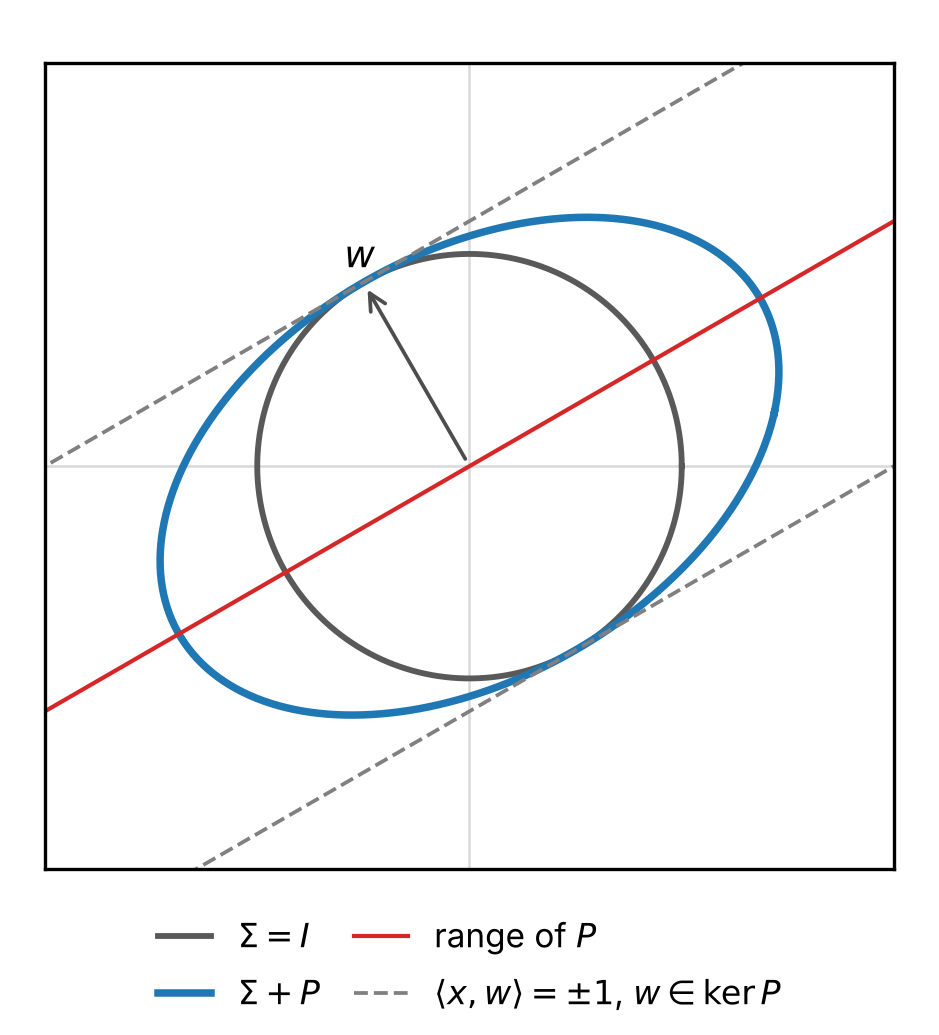
\includegraphics[width=0.5\textwidth]{fig-rank-deficient-step.png}
\caption{A rank-one Loewner step in the plane, from $\Sigma = I$ to $\Sigma + P$ with
$P = \tfrac32\,uu^{\tp}$, $u = (\cos 30^\circ, \sin 30^\circ)$: the apertures $\{x : \langle x, \Sigma^{-1}x\rangle \le 1\}$ of the two
matrices. The aperture widens along the range $\RR u$ of $P$. Its extent in a unit direction $w$ of
% Round 2 (presentation review), item 10: "unit" direction, which the tangent lines need.
the null space $\ker P$, which is $\langle w, \Sigma w\rangle^{1/2}$, is unchanged, so both ellipses touch the
lines $\langle x, w\rangle = \pm 1$. When the kernels depend on $\Sigma$ through one function $g$,
continuous at $0$ with $g(0) = 0$, Theorem~\ref{thm:rank-deficient-step} says that an increment of
such a step that is a probability measure is a centred Gaussian law carried by $\RR u$, the point
mass $\delta_0$ when $g \equiv 0$. Drawn by a script deposited with the paper.}
\label{fig:rank-deficient-step}
\end{figure}

% shared with blueprint thm:affine-rigidity
\begin{theorem}[affine rigidity: the affine Gaussian scale space]\label{thm:affine-rigidity}
Let $d \ge 2$. A family $(\mu_{\Sigma,\Sigma'})$ is an affine cascade family in dimension $d$ if
and only if it is the affine Gaussian scale space with some constant $b > 0$
(\ref{eq:affine-gaussian}). In particular the kernel from scale zero at $I$ of an affine cascade
family in dimension $d \ge 2$ is a centred Gaussian law with covariance a positive multiple of $I$,
and no other probability law on $\RR^d$ is the kernel $\mu_I$ of one.
\end{theorem}

Read against Theorem~\ref{thm:isotropic-classification} and Proposition~\ref{prop:isotropic-corner}(1),
the theorem says that for $d \ge 2$ no isotropic family with a non-Gaussian kernel is, after a change
of gauge, the slice of an affine cascade family, since the kernel $\mu_I$ of an affine cascade family
is Gaussian. The proof turns on the single step.

% shared with blueprint thm:rank-deficient-step
\begin{theorem}[one rank-deficient step forces the Gaussian]\label{thm:rank-deficient-step}
Let $d \ge 2$ and let $g : [0,\infty) \to [0,\infty)$ be continuous at $0$ with $g(0) = 0$.
Suppose there are $\Sigma \in \PD(d)$, $P \in \PSD(d)$ with $0 < \rank P < d$, and a probability
measure $\rho$ on $\RR^d$ with
\begin{equation}\label{eq:one-step}
  e^{-g(\langle\omega,(\Sigma+P)\omega\rangle)}
   = e^{-g(\langle\omega,\Sigma\omega\rangle)}\,\widehat\rho(\omega)
   \qquad (\omega \in \RR^d).
\end{equation}
Then $g(u) = b\,u$ with $b = g(1) \ge 0$, and $\rho$ is the centred Gaussian law with covariance
$2bP$. Conversely, if $g(u) = bu$ with $b \ge 0$, then \ref{eq:one-step} holds with that Gaussian
$\rho$ for every $\Sigma, P \in \PSD(d)$.
\end{theorem}

The hypotheses are about one step alone: $\rho$ is any probability measure, and $g$ is any
nonnegative function continuous at $0$ with $g(0) = 0$, whether or not
$e^{-g(\langle\omega,\Sigma\omega\rangle)}$ is a characteristic function. A step of full rank widens
the aperture in every direction, and $\ker P = \{0\}$ leaves the subspace argument nothing to act
on. Whether such a step can have a probability measure as its increment depends on $g$: for the
\Matern{} orbit no full-rank step can (Proposition~\ref{prop:matern-steps}), and for the isotropic
stable orbit the steps of a cone can (Proposition~\ref{prop:stable-step-cone}).

The proofs of the two theorems rest on three lemmas, proved in Appendix~\ref{app:classical}.

% shared with blueprint lem:charfn-one-on-subspace
\begin{lemma}[a characteristic function equal to $1$ on a subspace]\label{lem:charfn-one-on-subspace}
Let $\rho$ be a probability measure on $\RR^d$ and $H \subseteq \RR^d$ a linear subspace with
$\widehat\rho(\eta) = 1$ for every $\eta$ in a neighbourhood of $0$ in $H$. Then $\rho$ is carried
by the orthogonal complement $H^\perp$, and $\widehat\rho(\omega + \eta) = \widehat\rho(\omega)$ for all
$\omega \in \RR^d$ and $\eta \in H$. In particular, if $\widehat\rho = 1$ near $0$ then
$\rho = \delta_0$.
\end{lemma}

The second statement of the lemma also follows from a general fact. For a positive definite function
$f$ with $f(0) = 1$, the set $G_f$ where $|f| = 1$ is a group, and $f(x + y) = f(x)f(y)$ for
$x \in G_f$ and every $y$ (\sscite{sasvari2013multivariate}, Cor.~1.4.13, p.~29). For $f = \widehat\rho$,
every $\eta \in H$ is a sum of points of the neighbourhood where $\widehat\rho = 1$, so the product rule
gives $\widehat\rho(\eta) = 1$. Then $\widehat\rho(\omega + \eta) = \widehat\rho(\eta)\widehat\rho(\omega) =
\widehat\rho(\omega)$.

The next lemma reduces an affine cascade family to one function of one variable. Covariance makes the kernels from scale zero depend on $\Sigma$ through $\langle\omega,\Sigma\omega\rangle$. Along the ray of $I$ the
cascade (K1) and continuity (K2) exclude a first zero of the transform, so the transform is positive
and $g$ is its negative logarithm. Nondegeneracy (K4) makes $g \not\equiv 0$.

% shared with blueprint lem:affine-reduction
\begin{lemma}[reduction to one function]\label{lem:affine-reduction}
Let $(\mu_{\Sigma,\Sigma'})$ be an affine cascade family in dimension $d$. There is a continuous
$g : [0,\infty) \to [0,\infty)$ with $g(0) = 0$ and $g \not\equiv 0$ such that
\begin{equation}\label{eq:affine-reduction}
  \widehat\mu_\Sigma(\omega) = e^{-g(\langle\omega,\Sigma\omega\rangle)}
  \qquad (\Sigma \in \PSD(d),\ \omega \in \RR^d),
\end{equation}
and for every pair $\Sigma \le \Sigma'$
\begin{equation}\label{eq:affine-increment}
  \widehat\mu_{\Sigma,\Sigma'}(\omega)
   = \exp\bigl[-g(\langle\omega,\Sigma'\omega\rangle) + g(\langle\omega,\Sigma\omega\rangle)\bigr] .
\end{equation}
\end{lemma}

A single Loewner step turns \ref{eq:affine-increment} into a functional equation for $g$, which the next
lemma solves.

% shared with blueprint lem:single-ratio-cauchy
\begin{lemma}[one ratio forces linearity]\label{lem:single-ratio-cauchy}
Let $g : [0,\infty) \to [0,\infty)$ be continuous at $0$ with $g(0) = 0$, and let $a > 1$ be such
that
\begin{equation}\label{eq:single-ratio}
  g(au + w) - g(u + w) = g(au) - g(u) \qquad \text{for all } u > 0,\ w \ge 0 .
\end{equation}
Then $g(u) = b\,u$ for every $u \ge 0$, with $b = g(1) \ge 0$.
\end{lemma}

With the three lemmas the two theorems are proved, the single step first.



% proof of thm:rank-deficient-step
\begin{proof}[Proof of Theorem~\ref{thm:rank-deficient-step}]
\emph{Transport to the identity and diagonalize.} Put $P' := \Sigma^{-1/2}P\Sigma^{-1/2} \in
\PSD(d)$, of rank $r := \rank P$, and choose $Q \in \Orth(d)$ with
$Q^{\tp}P'Q = \diag(p_1,\dots,p_r,0,\dots,0)$, $p_i > 0$. For $\omega = \Sigma^{-1/2}Q\zeta$ one
has $\langle\omega,\Sigma\omega\rangle = |\zeta|^2$ and
$\langle\omega,P\omega\rangle = \sum_{i \le r}p_i\zeta_i^2$. Let $C := Q^{\tp}\Sigma^{-1/2}$ and
$\rho' := C_*\rho$, so that $\widehat{\rho'}(\zeta) = \widehat\rho(C^{\tp}\zeta)
= \widehat\rho(\Sigma^{-1/2}Q\zeta)$. Dividing \ref{eq:one-step} by
$e^{-g(\langle\omega,\Sigma\omega\rangle)}$, which has no zero,
\[
  \widehat{\rho'}(\zeta) = \exp\Bigl[-g\Bigl(|\zeta|^2 + \sum_{i\le r}p_i\zeta_i^2\Bigr)
     + g\bigl(|\zeta|^2\bigr)\Bigr] .
\]

\emph{The subspace.} On $H := \{\zeta : \zeta_1 = \dots = \zeta_r = 0\}$, of dimension
$d - r \ge 1$, the exponent vanishes and $\widehat{\rho'} = 1$. By
Lemma~\ref{lem:charfn-one-on-subspace}, $\widehat{\rho'}(\zeta + \eta) = \widehat{\rho'}(\zeta)$ for
$\eta \in H$. Take $\zeta = t e_1$ with $t > 0$ and $\eta \in H$ arbitrary, and put
$a := 1 + p_1 > 1$, $u := t^2$, $w := |\eta|^2$: the invariance reads
\[
  g(au + w) - g(u + w) = g(au) - g(u) ,
\]
and as $t$ ranges over $(0,\infty)$ and $\eta$ over $H \ne \{0\}$, the pair $(u,w)$ ranges over
$(0,\infty) \times [0,\infty)$. That is \ref{eq:single-ratio}, and
Lemma~\ref{lem:single-ratio-cauchy} gives $g(u) = bu$ with $b = g(1) \ge 0$.

\emph{The increment, and the converse.} Now \ref{eq:one-step} reads
$\widehat\rho(\omega) = e^{-b\langle\omega,P\omega\rangle}$, the characteristic function of the
centred Gaussian law with covariance $2bP$ (the law of $(2bP)^{1/2}Z$, $Z$ standard normal on
$\RR^d$); by uniqueness of the transform $\rho$ is that law. Conversely, for $g(u) = bu$ the
exponents in \ref{eq:one-step} are linear in the matrix, and the same Gaussian satisfies it for any
$\Sigma, P \in \PSD(d)$.
\end{proof}

% proof of thm:affine-rigidity
\begin{proof}[Proof of Theorem~\ref{thm:affine-rigidity}]
\emph{Necessity.} By Lemma~\ref{lem:affine-reduction} there is a continuous $g \ge 0$ with $g(0) = 0$
and $g \not\equiv 0$ satisfying \ref{eq:affine-reduction} and \ref{eq:affine-increment}. Take
$\Sigma = I$ and $P = e_1e_1^{\tp}$, of rank $1 < d$, and $\rho := \mu_{I,I+P}$, a probability
measure. Then \ref{eq:affine-increment} at the pair $I \le I + P$, multiplied by
$e^{-g(|\omega|^2)}$, is \ref{eq:one-step}. So Theorem~\ref{thm:rank-deficient-step} gives $g(u) = bu$,
and $b > 0$ because $g \not\equiv 0$. Now \ref{eq:affine-increment} is \ref{eq:affine-gaussian} for
every pair, and by uniqueness of the transform each $\mu_{\Sigma,\Sigma'}$ is the stated Gaussian.

\emph{Sufficiency.} Let $b > 0$ and let $\mu_{\Sigma,\Sigma'}$ be the centred Gaussian with
covariance $2b(\Sigma'-\Sigma)$, which exists for every positive semidefinite covariance as the law
of $(2b(\Sigma'-\Sigma))^{1/2}Z$. Its transform is \ref{eq:affine-gaussian}. The axioms of
Definition~\ref{def:affine-cascade-family} hold. (K1): the transform
at $\Sigma = \Sigma'$ is $1$, and the exponents of $\mu_{\Sigma',\Sigma''}$ and
$\mu_{\Sigma,\Sigma'}$ add to that of $\mu_{\Sigma,\Sigma''}$; by uniqueness of the transform,
$\mu_{\Sigma,\Sigma} = \delta_0$ and the convolution identity holds. (K2): the transform is
continuous in $(\Sigma,\Sigma')$. (K3): $\widehat{A_*\mu_{\Sigma,\Sigma'}}(\omega)
= e^{-b\langle A^{\tp}\omega,(\Sigma'-\Sigma)A^{\tp}\omega\rangle}
= e^{-b\langle\omega,(A\Sigma'A^{\tp} - A\Sigma A^{\tp})\omega\rangle}$. (K4):
$\widehat\mu_{0,I}(e_1) = e^{-b} \ne 1$.

\emph{The last clause.} By necessity, $\widehat\mu_I(\omega) = e^{-b|\omega|^2}$ with $b > 0$.
\end{proof}

The proof uses (K1)--(K4) through Lemma~\ref{lem:affine-reduction} and then one step of the
cascade, $I \le I + e_1e_1^{\tp}$, and of $g$ it needs only continuity at $0$ and $g \ge 0$.

% Round 3 (report B, part 3 (ii); the author's decision D12, PLAN-review-response-paper.md R3.0):
% where continuity enters the rigidity, with the family that shows it is needed there.
Continuity (K2) enters that proof in Lemma~\ref{lem:affine-reduction}, twice: to exclude a first zero of
the transform along the ray of $I$, and to reach the kernels at the singular apertures. The cascade and
the dilations do the first without it, by making $\mu_I$ self-decomposable, and the second cannot be
done without it.

% shared with blueprint prop:affine-rigidity-boundary
\begin{proposition}[continuity is needed only at the boundary of $\PSD(d)$]\label{prop:affine-rigidity-boundary}
Let $d \ge 2$, and let $(\mu_{\Sigma,\Sigma'})$ be probability measures on $\RR^d$, indexed by the pairs
$\Sigma \le \Sigma'$ in $\PSD(d)$, that satisfy (K1), (K3) and (K4) of Definition~\ref{def:affine-cascade-family}, but
not necessarily (K2).
\begin{enumerate}
\item \emph{(Between positive definite apertures.)} There is $b > 0$ such that for every $\Sigma \in \PD(d)$
the kernel from scale zero $\mu_\Sigma$ is the centred Gaussian law with covariance $2b\Sigma$, and for every
pair $\Sigma \le \Sigma'$ in $\PD(d)$ the increment $\mu_{\Sigma,\Sigma'}$ is the centred Gaussian law with
covariance $2b(\Sigma' - \Sigma)$. In particular $\mu_I$ is the centred Gaussian law with covariance $2bI$.
\item \emph{(At the boundary.)} Let $b > 0$ and $0 \le \theta_0 < 1$, put $\theta(\Sigma) := 1$ for
$\Sigma \in \PD(d)$ and $\theta(\Sigma) := \theta_0$ for singular $\Sigma \in \PSD(d)$, and for
$\Sigma \le \Sigma'$ let $\mu_{\Sigma,\Sigma'}$ be the centred Gaussian law with covariance
$2b(\theta(\Sigma')\Sigma' - \theta(\Sigma)\Sigma)$. This covariance is positive semidefinite for every pair,
and the family satisfies (K1), (K3) and (K4) and agrees with the affine Gaussian scale space with constant
$b$ on the pairs in $\PD(d)$. Its kernel from scale zero at a nonzero singular $P$ has covariance
$2b\theta_0P$, so the family is not an affine Gaussian scale space, and it does not satisfy (K2).
\end{enumerate}
\end{proposition}

\begin{proof}
\emph{(1).} Let $\vartheta(u) := \widehat\mu_I(\sqrt u\,e_1)$, $u \ge 0$. As in the first step of the proof of
Lemma~\ref{lem:affine-reduction}, which reads only (K3), $\mu_I$ is rotation invariant,
$\widehat\mu_I(\omega) = \vartheta(|\omega|^2)$, and $\vartheta$ is continuous and real with $\vartheta(0) = 1$
and $|\vartheta| \le 1$. For $\Sigma \in \PD(d)$, (K3) with $A = \Sigma^{1/2}$ gives
$\widehat\mu_\Sigma(\omega) = \vartheta(\langle\omega,\Sigma\omega\rangle)$. For $0 < c < 1$, (K1) at
$0 \le c^2I \le I$ gives $\mu_I = \mu_{c^2I} * \mu_{c^2I,I}$, and (K3) with $A = cI$ at the pair $(0, I)$
gives $\mu_{c^2I} = (cI)_*\mu_I$. So $\mu_I$ is self-decomposable \ref{eq:self-decomposable}, and its
transform has no zero (Proposition~\ref{prop:gw-ray-families}(1)). Being real and continuous with $\vartheta(0) = 1$,
$\vartheta$ is then positive, and $g := -\log\vartheta$ is continuous, nonnegative and $g(0) = 0$. If
$g \equiv 0$, then $\widehat\mu_I \equiv 1$ and $\mu_I = \delta_0$ (Lemma~\ref{lem:charfn-one-on-subspace}), against
(K4). Put $P := e_1e_1^{\tp}$, of rank $1 < d$. (K1) at $0 \le I \le I + P$ gives
$\mu_{I+P} = \mu_{I,I+P} * \mu_I$, which is \ref{eq:one-step} with $\Sigma = I$ and $\rho = \mu_{I,I+P}$. So
Theorem~\ref{thm:rank-deficient-step} gives $g(u) = bu$ with $b = g(1)$, and $b > 0$ as $g \not\equiv 0$. Hence
$\widehat\mu_\Sigma(\omega) = e^{-b\langle\omega,\Sigma\omega\rangle}$ for $\Sigma \in \PD(d)$, the transform of
the centred Gaussian law with covariance $2b\Sigma$. For $\Sigma \le \Sigma'$ in $\PD(d)$, (K1) at
$0 \le \Sigma \le \Sigma'$ gives $\widehat\mu_{\Sigma'} = \widehat\mu_{\Sigma,\Sigma'}\,\widehat\mu_\Sigma$, and as
$\widehat\mu_\Sigma$ has no zero, $\widehat\mu_{\Sigma,\Sigma'}(\omega) = e^{-b\langle\omega,(\Sigma'-\Sigma)\omega\rangle}$.
The uniqueness of the transform names each law.

\emph{(2), the covariances.} Let $\Sigma \le \Sigma'$ and $D := \theta(\Sigma')\Sigma' - \theta(\Sigma)\Sigma$. If
$\Sigma$ is definite, so is $\Sigma' \ge \Sigma$, and $D = \Sigma' - \Sigma \ge 0$. If both are singular,
$D = \theta_0(\Sigma' - \Sigma) \ge 0$. If $\Sigma$ is singular and $\Sigma'$ definite,
$D = \Sigma' - \theta_0\Sigma = (\Sigma' - \Sigma) + (1 - \theta_0)\Sigma \ge 0$. So each $\mu_{\Sigma,\Sigma'}$ exists,
with transform $e^{-b\langle\omega,D\omega\rangle}$.

\emph{(2), the axioms.} (K1): at $\Sigma = \Sigma'$, $D = 0$. For $\Sigma \le \Sigma' \le \Sigma''$ the
matrices $D$ of the pairs $(\Sigma, \Sigma')$ and $(\Sigma', \Sigma'')$ add to that of $(\Sigma, \Sigma'')$, so the
transforms multiply and the uniqueness of the transform gives the cascade identity. (K3): an $A \in \GL(d)$
preserves rank, so $\theta(A\Sigma A^{\tp}) = \theta(\Sigma)$, and $A_*\mu_{\Sigma,\Sigma'}$, the centred Gaussian
law with covariance $2bADA^{\tp}$, is $\mu_{A\Sigma A^{\tp},\,A\Sigma'A^{\tp}}$. (K4): $\theta(0)\,0 = 0$, so
$\mu_{0,I}$ has covariance $2bI$ and is not $\delta_0$. On a pair in $\PD(d)$, $D = \Sigma' - \Sigma$, which is
\ref{eq:affine-gaussian}. For a nonzero singular $P$, $\mu_{0,P}$ has covariance $2b\theta_0P$. An affine Gaussian scale space
with this $\mu_{0,I}$ has the constant $b$, by \ref{eq:affine-gaussian} at the pair $(0, I)$, and its kernel at $P$
has covariance $2bP \ne 2b\theta_0P$, as $\theta_0 < 1$ and $P \ne 0$. Finally, $P + n^{-1}I$ is
definite and tends to $P$, while for $\omega$ with $P\omega \ne 0$,
$\widehat\mu_{0,P+n^{-1}I}(\omega) = e^{-b\langle\omega,(P+n^{-1}I)\omega\rangle} \to e^{-b\langle\omega,P\omega\rangle}
\ne e^{-b\theta_0\langle\omega,P\omega\rangle} = \widehat\mu_{0,P}(\omega)$. So (K2) fails at the pair $(0, P)$.
\end{proof}

So by Proposition~\ref{prop:affine-rigidity-boundary}, on the positive definite apertures the axioms need no
continuity, and Iijima's, as reported in
Remark~\ref{rem:lindeberg}, list none. Continuity fixes only the kernels and increments at the singular
apertures.

\begin{remark}[positivity carries weight]\label{rem:positivity}
The classification theorems of this paper use positivity: their kernels and increments are probability
measures. In the rigidity it enters twice: through
Lemma~\ref{lem:charfn-one-on-subspace}, which says that a probability measure whose transform is $1$ on a
subspace is carried by its orthogonal complement, and through the sign of the function $g$ of
Lemma~\ref{lem:affine-reduction}. That function is nonnegative because the transform of a probability
law has modulus at most $1$, and Lemma~\ref{lem:single-ratio-cauchy} uses the sign, with continuity at
$0$, in place of every other regularity in Cauchy's equation. Without
positivity the increments need not be signed measures: across shapes the increment of the \Matern{} orbit of
index $1$ is not even a finite signed measure (Proposition~\ref{prop:matern-negative-mass}(3)).
\end{remark}

The theorem holds on operators too. The passage from operators to kernels
(Lemma~\ref{lem:operators-to-kernels}) has a converse, from a family of kernels to a
family of operators continuous in $L^1$ (Lemma~\ref{lem:kernels-to-operators}, both in
Appendix~\ref{app:classical}), and the two together carry the rigidity over.

% shared with blueprint thm:affine-rigidity-operators+3a6bc0ff67da
\begin{theorem}[affine rigidity on operators]\label{thm:affine-rigidity-operators}
Let $d \ge 2$. A family $(\Phi_{\Sigma,\Sigma'})$ of linear operators on $L^1(\RR^d)$, indexed by the
pairs $\Sigma \le \Sigma'$ in $\PSD(d)$, is a $(\GL(d), \text{Loewner})$-cascade family of operators
(Definition~\ref{def:gw-cascade-family}(1)) if and only if there is $b > 0$ such that
$\Phi_{\Sigma,\Sigma'}f = \mu_{\Sigma,\Sigma'} * f$ for every pair and every $f \in L^1(\RR^d)$, where
$(\mu_{\Sigma,\Sigma'})$ is the affine Gaussian scale space with constant $b$
(Definition~\ref{def:affine-cascade-family}, \ref{eq:affine-gaussian}). The constant $b$ is then unique.
\end{theorem}

\begin{proof}
\emph{Necessity.} By Lemma~\ref{lem:operators-to-kernels}(4) the measures $\mu_{\Sigma,\Sigma'}$
with $\Phi_{\Sigma,\Sigma'}f = \mu_{\Sigma,\Sigma'} * f$ form an affine cascade family in dimension
$d$, and by Theorem~\ref{thm:affine-rigidity} it is the affine Gaussian scale space with some $b > 0$.

\emph{Sufficiency.} By Theorem~\ref{thm:affine-rigidity} the affine Gaussian scale space with constant
$b > 0$ is an affine cascade family, that is a $(\GL(d), \text{Loewner})$-cascade family of kernels,
and $(\GL(d), \text{Loewner})$ is a wedge datum (Definition~\ref{def:gw-cascade-family}). By
Lemma~\ref{lem:kernels-to-operators}(2) the operators $f \mapsto \mu_{\Sigma,\Sigma'} * f$ form a
$(\GL(d), \text{Loewner})$-cascade family of operators.

\emph{Uniqueness of $b$.} If $\Phi_{0,I}$ is convolution by the Gaussian laws of constants $b$ and
$b'$, the uniqueness clause of Lemma~\ref{lem:operators-to-kernels}(1) makes the two laws equal, and their
transforms \ref{eq:affine-gaussian} at $\Sigma = 0$, $\Sigma' = I$ and $\omega = e_1$ give
$e^{-b} = e^{-b'}$.
\end{proof}

\subsection{Prior art, and the relation to the line}\label{sec:classical-prior-art}

This subsection places Theorem~\ref{thm:affine-rigidity} among the axiomatics of scale space and the
characterizations of the normal law. The family it selects is classical, and so is its covariance
under linear maps. The morphological axiomatics reads ``affine'' in another sense, and the
$\alpha$-scale spaces admit the stable laws, which the classical corner removes. As a
characterization of the normal law its core is Kelker's lemma (Remark~\ref{rem:kelker}), and as an
axiomatic derivation it stands beside Lindeberg's (Remark~\ref{rem:lindeberg}).
Remark~\ref{rem:classical-line} reads the scheme on the line.

The affine Gaussian scale space is classical. Lindeberg and G\aa{}rding define it in the plane by
the Gaussian kernels of the positive semidefinite covariance matrices, and it is closed under linear changes of
the image coordinates: an invertible $B$ moves the matrix by $\Sigma \mapsto B\Sigma B^{\tp}$
% Round 3 (content review), A.R10: p. 10 and the equation numbers are the KTH report's, not the
% journal article's; the held copy is the report. Both are dropped, and the next sentence's "the same
% page" (report p. 10, section 4.1, read again for this edit) becomes the section.
(\sscite{lindeberg1997shape}, \S\S4 and~4.1). The rotationally symmetric
linear scale space has that closure only for rotations and uniform rescalings (the same source, \S4.1).

The word ``affine'' has another sense in the morphological axiomatics of Alvarez, Guichard, Lions
and Morel. There the scale stays a scalar $t$, and a linear map $A$ of the image is required to be
absorbed by a change of that scalar, $AT_{t'} = T_tA$ for some $t'(t, A)$
(\sscite{alvarez1993axioms}, [Projection invariance], p.~206). In the plane, with grey-scale and
scale invariance among the hypotheses, this leaves the nonlinear affine morphological scale space
$\partial u/\partial t = |Du|\,(t\operatorname{curv}(u))^{1/3}$ (Thm.~5(iii), p.~229). Their
linear multiscale analyses with isometric invariance are the heat equation, up to a rescaling of
$t$ (Thm.~3, p.~214), and its rotationally symmetric kernels are not closed under an anisotropic
map. Indexing the kernels by matrices is what lets a linear, positive family be covariant under
$\GL(d)$. With the cascade along the whole Loewner order and $d \ge 2$,
Theorem~\ref{thm:affine-rigidity} says that the Gaussian is then the only one.

The other neighbours are the axiomatics that admit the stable laws. For linear, even, recursive
and scale-invariant filters on the line, Pauwels, Van Gool, Fiddelaers and Moons obtain the
transforms $e^{-a|\omega|^\alpha t}$, $\alpha > 0$, so that these conditions do not single out the
Gaussian (\sscite{pauwels1995extended}, p.~694). The kernels have zero crossings for $\alpha > 2$
(pp.~694--695). Duits, Florack, de Graaf and ter Haar Romeny write this class on $\RR^d$ as the
$\alpha$ scale spaces generated by $-(-\Delta)^\alpha$ (\sscite{duits2004axioms}, (25), p.~277),
whose transforms are $e^{-s|\omega|^{2\alpha}}$. Under positivity the parameter lies in $(0, 1]$,
with $\alpha = \tfrac12$ the Poisson and $\alpha = 1$ the Gaussian scale space (p.~267). Pauwels'
$\alpha$ is the stable index of this paper, and the $\alpha$ of Duits et al.\ is half of it. Where they
are positive, the kernels of both classes are the isotropic stable laws, which the isotropic theory contains. For $d \ge 2$ the classical corner removes them: by Theorem~\ref{thm:affine-rigidity} no stable law other than the Gaussian is the
kernel $\mu_I$ of an affine cascade family. Felsberg and Sommer show that the planar Poisson kernel
satisfies Iijima's axioms for a scalar scale (\sscite{felsberg2004monogenic}, Thm.~1, p.~7), and in an
earlier outlook propose a $2 \times 2$ scaling matrix in place of that scale
(\sscite{felsberg2001scale}, \S5, p.~130). The elliptical Poisson orbit is the stable orbit of
index~$1$, whose positive increments form the cone of Proposition~\ref{prop:stable-step-cone}(1), with
no rank-deficient step in it (Theorem~\ref{thm:rank-deficient-step}).

Two earlier results bear on Theorem~\ref{thm:affine-rigidity} directly: Kelker's characterization of
the normal law, which is its core (Remark~\ref{rem:kelker}), and Lindeberg's derivation of the same
family from other axioms (Remark~\ref{rem:lindeberg}).

\begin{remark}[Kelker's lemma]\label{rem:kelker}
A rotation-invariant law with independent coordinates is normal. In the plane this is the
Herschel--Maxwell theorem (\sscite{bryc1995normal}, Thm.~0.0.1, p.~1).
% Bryc read at the page (Q-0294; records/affine/READING-bryc1995normal.md).
In every dimension it is Kelker's lemma, proved for the centred laws whose transform has the form
$\psi(\langle\omega,\Sigma\omega\rangle)$ with $\Sigma$ diagonal, of which the rotation-invariant
laws are the case $\Sigma = I$ (\sscite{kelker1970distribution}, Lemma~5, p.~423). Fang, Kotz and Ng restate it with pairwise independence
(\sscite{fang1990symmetric}, Thm.~4.11, p.~106). The following sketch shows that it is the core of
Theorem~\ref{thm:affine-rigidity}. From the base $I - e_1e_1^{\tp}$ of an affine cascade family,
$\mu_I = \mu_{I - e_1e_1^{\tp}} * \mu_{I - e_1e_1^{\tp},\,I}$, and by
Lemma~\ref{lem:charfn-one-on-subspace} the first factor is carried by $e_1^\perp$ and the second by
the $e_1$-axis. So the first coordinate of $\mu_I$ is independent of the others.
% Round 3 (content review), B.S6: the step to mutual independence, and where the base lies.
By rotation invariance every coordinate is, so the transform factors over the coordinates. The
coordinates are then independent, and Kelker's lemma makes $\mu_I$ normal. The step used has a singular base, which lies
outside Theorem~\ref{thm:rank-deficient-step} and inside Definition~\ref{def:affine-cascade-family}. What the scale-space
setting adds is the single-step form, Theorem~\ref{thm:rank-deficient-step}. It reads one step
$\Sigma \to \Sigma + P$, with $\Sigma$ positive definite and $P$ singular, whose increment is any
probability measure. And $e^{-g(\langle\omega,\Sigma\omega\rangle)}$ need not be a characteristic
function there. Kelker, Fang, Kotz and Ng, Bryc,
and Cambanis, Huang and Simons characterize the normal law among the \emph{elliptically contoured}
laws, the linear images of rotation-invariant laws shifted by a vector, by
properties of one vector, such as independent coordinates, conditional laws, quadratic forms or
marginal densities (\sscite{kelker1970distribution}, Lemma~5, p.~423, Thm.~7 and Lemma~8,
pp.~424--426; \sscite{cambanis1981theory}, \S5, pp.~379--384). Khatri and Mukerjee characterize the
normal law by the law of one quadratic form, and Anderson and Fang by the independence of two complementary
quadratic forms of one spherical vector (\sscite{khatri1987characterization}, Thm.~1, p.~187;
\sscite{anderson1987cochran}, Thm.~1, p.~309). Kelker's route, and that of Cambanis, Huang and
Simons, goes through Cauchy's equation for the generator, as Lemma~\ref{lem:single-ratio-cauchy} does
(\sscite{kelker1970distribution}, p.~423; \sscite{cambanis1981theory}, Thm.~6, pp.~379--380).
% Q-0314: Khatri-Mukerjee and Anderson-Fang read at the page (READING-khatri1987characterization.md,
% READING-anderson1987cochran.md): one-vector characterizations, by moment series and through
% Lukacs's gamma characterization; the TODO(source) is closed, and the claim stays "not found in the
% sources read". The earlier text had lost the subject of the Cauchy sentence inside that comment.
% Writing-rules follow-up (2026-10-14; PASS-writing-rules-affine.md, owed item 3): that claim, and
% "None of these sources relates two scale matrices of one generator by a convolution", are gone
% (the author's direction against novelty claims); the contrast stays in "by properties of one vector".
% Q-0317 (the blind register review, section 3 flag 13): the subject of the next sentence had been
% swallowed into this comment's last line; it is restored on its own line.
Where the Gaussian has the whole Loewner order, the non-Gaussian orbits keep cones of full-rank steps
(Propositions~\ref{prop:stable-step-cone} and~\ref{prop:orbit-step-cone}).
% Q-0309 (fix group 5): Cambanis-Huang-Simons read at the page by Q-0308
% (records/affine/READING-cambanis1981theory.md): non-proportional scale matrices occur there only as
% non-uniqueness (Thm. 3(i), pp. 372-373); no statement on sums or convolutions of elliptical
% vectors. Fang-Kotz-Ng 4.3 (READING-fang1990symmetric.md) and Bryc (READING-bryc1995normal.md) as
% before. The review's lead (flag 46) is not in these sources; PRIOR-ART-novelty-claims.md lists
% what a referee could still name (Anderson-Fang, Khatri-Mukerjee; Kelker pp. 424-430).
% Q-0312: Kelker pp. 424-430 read on the images (READING-kelker1970distribution.md, section 5):
% regression, conditional covariance (Thm. 7), conditional normality (Lemma 8), Schoenberg, norms
% and quadratic forms, all of one vector; nothing relates two scale matrices by a convolution.
A form without any
covariance group, with the Darmois--Skitovich theorem (\sscite{skitovich1954linear}, Thm.~2,
p.~190) in place of Kelker's lemma, is open
problem~\ref{prob:no-covariance} of \S\ref{sec:open-problems}.
\end{remark}

\begin{remark}[Lindeberg's and Iijima's derivations]\label{rem:lindeberg}
Lindeberg \sscite{lindeberg2011generalized} assumes a semigroup in a scalar scale $s$, strong
continuity with a Sobolev regularity condition, and non-enhancement of local extrema. From these,
his Theorem~5 (p.~42) obtains a local generator of order two with a positive semidefinite matrix
$\Sigma_0$, and the affine Gaussian scale space is its positive definite, mirror-symmetric case
(\S4.1.2, p.~45). Positivity, unit mass and closure under affine maps are properties of his
solution, not axioms, and non-enhancement is what removes the stable laws (\S2, p.~39).
Theorem~\ref{thm:affine-rigidity} takes as axioms positivity, a cascade over Loewner-ordered pairs
of matrices, continuity in the pair, nondegeneracy at one pair and $\GL(d)$-covariance, for $d \ge 2$.
The two results have different shapes. His classifies all non-enhancing continuous semigroups, one
Gaussian ray $\{s\Sigma_0\}$ for each matrix $\Sigma_0$ and drift, with the affine group acting on
the rays afterwards. This one is a rigidity statement for one two-parameter family with a group
action. Neither implies the other from its own hypotheses: his axioms have no positivity and no
order on matrices, and this one has no non-enhancement and does not cover $d = 1$. The order appears
in his later work as the meaning of a larger matrix scale (\sscite{lindeberg2013computational}, fn.~7,
p.~594). On the ray from
$\Sigma = 0$ to $\Sigma' = s\Sigma_0$, the kernel of \ref{eq:affine-gaussian} with $b = \tfrac12$ is
his kernel (45), p.~44, with zero drift.

Iijima's axioms of 1962 and 1963, as Weickert, Ishikawa and Imiya report them
(\sscite{weickert1999linear}, p.~241), are closer in form. The scale is a positive definite
$2 \times 2$ matrix. The transformations are linear, translation invariant and positive, and they are
closed under every invertible linear map. Any two of them compose to a third member of the family,
with no order on the scales. These axioms give the affine Gaussian scale space. For a scalar scale,
Felsberg and Sommer find that Iijima's uniqueness proof assumes implicitly a transform continuously
differentiable at the origin, which that of the Poisson kernel is not (\sscite{felsberg2004monogenic},
p.~8, and n.~2, p.~24). As hypotheses the two
sets are incomparable. Iijima composes every pair of scales and asks that the composite be in the
family. Theorem~\ref{thm:affine-rigidity} indexes its increments by pairs, does not ask that they be
members, and asks for them only from a matrix to a larger one in the Loewner order.
% Round 3 (content review), B.S2 (the author's decision D12): the pointer to Proposition 3.11.
It adds continuity in the pair, which is needed only at the singular matrices
(Proposition~\ref{prop:affine-rigidity-boundary}). It holds for every $d \ge 2$.
\end{remark}

\begin{remark}[relation to the line]\label{rem:classical-line}
At $d = 1$, $\PSD(1) = [0,\infty)$, and the Loewner order and the ray order are both the order of
the half-line. The similarities are all of $\GL(1)$, so the four corners of
Definition~\ref{def:gw-cascade-family} coincide, and every pair is on the slice. By
Proposition~\ref{prop:isotropic-corner}(1) and (2) with $d = 1$, the families of the scheme are then
the isotropic families in dimension $1$, read in the variance gauge, and those are the line's
families of Definition~\ref{def:line-family} on kernels \prog{Iso}{Rem.~3.26}.
So on the
line the classical corner is the line's theory with its gauge fixed, and the kernel $\mu_1$ at
scale $1$ of such a family can be any symmetric self-decomposable law other than $\delta_0$, and
only such a law (Theorem~\ref{thm:line-classification}). On the line the relabelling of the scales
is free, and the gauge $\chi$ of Theorem~\ref{thm:line-classification} is part of the answer. For $d \ge 2$ and
$G = \GL(d)$ the group acts transitively on $\PD(d)$, and Lemma~\ref{lem:affine-gauge} forces the
parametrization up to one constant. The rigidity belongs to dimension $d \ge 2$:
Theorem~\ref{thm:rank-deficient-step} needs a step with $0 < \rank P < d$, which the line does not
have.
\end{remark}
